% !TEX root = ../main.tex

\section{Introduction}

%Note: talk about why it matters to fix ERC20 implementation: cause it is supported by the eco-system, a fixed erc20 implementation can be added to any DEX.


Ethereum is a public blockchain proposed in 2013, deployed in 2015~\cite{Ref00}, and has the second largest market cap at the time of writing\footnote{[2019-02-11] \url{https://coinmarketcap.com/currencies/ethereum/}}. It has a large development community which track enhancements and propose new ideas.\footnote{[2019-02-11] \url{https://www.coindesk.com/data}} Ethereum enables decentralized applications (\dapps) to be deployed and executed. \dapps can accept and transfer Ethereum's built-in currency (ETH) or might issue their own custom currency-like tokens for specific purposes. Tokens might be currencies with different properties than ETH, they may be required for access to a \dapp's functionality or they might represent ownership of some off-blockchain asset. It is beneficial to have interoperable tokens with other \dapps and off-blockchain webapps, such as exchange services that allow tokens to be traded.

Toward this goal, the Ethereum project accepted a proposed standard (called ERC20~\cite{Ref08}) for a set of methods which standard-compliant tokens should implement. In terms of object oriented programming, ERC20 is an interface that defines abstract methods (name, parameters, return types) and provides guidelines on how the methods should be implemented, however it does not provide a actual concrete implementation (see Figure~\ref{fig:erc20api}). 

\begin{figure}[t!]
	\centering
	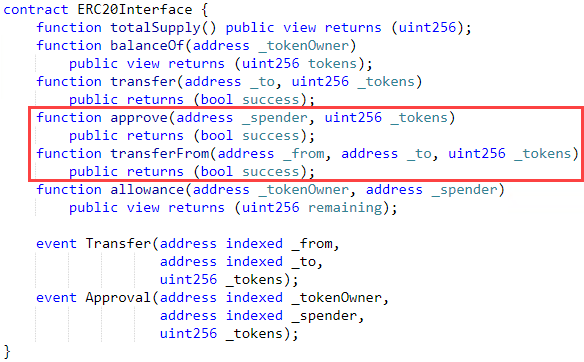
\includegraphics[width=1.0\linewidth]{figures/multiple_withdrawal_01.png}
	\caption{The ERC20 standard defines 6 methods and 2 events that must be implemented. Using \texttt{approve} and \texttt{transferFrom} in the existence of a race condition may lead to a \textit{``multiple withdrawal attack''}\label{fig:erc20api}}
\end{figure}

% the blockchain. Tokens are essential part of this ecosystem which define set of rules---known as API\footnote{Advanced Programming Interface.}---for standardizing interaction with smart contracts.\footnote{Types of transactions that execute as they are programmed by Ethereum scripting language (e.g., Solidity or Vyper)}. Therefore, any ERC20\footnote{ERC20 is title of the standard and it should be referred as EIP20 (which is the actual proposal for improvement). In this paper we use both ERC20 and EIP20 in one sense for simplicity.}-compliant application can interact with any ERC20 token for trading, swapping, exchanging, etc. For example, shares of company X can be represented as ERC20 tokens to be reusable by other smart contracts (e.g., online exchanges, automated payment systems, decentralized games, etc). Leveraging ERC20 token facilitates implementation of financial assets while raising some security concerns. ERC20 tokens are technically standardized version of smart contracts that could be similarly vulnerable to security flaws.

% Jeremy: This seems unnecessary:
%\begin{figure}[t]
%	\centering
%	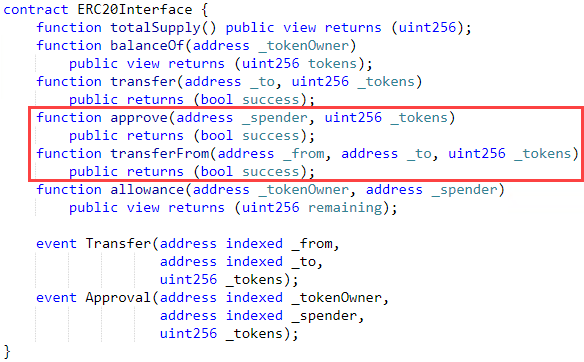
\includegraphics[width=1.0\linewidth]{figures/multiple_withdrawal_01.png}
%	\caption{Importance of ERC20 security in case of (1) digitizing share of company X (2) representing a fiat currency. In this case, smart contracts interact with two different ERC20 tokens which are repressing in sequence, a financial instrument and a non-collateralized stablecoin. Any security vulnerability in written code of ERC20 tokens, will impact security of related smart contracts and value of underlying assets.}
%\end{figure}

Since the introduction of ERC20 in November 2015, several vulnerabilities have been discovered. In October 2017, a security issue called \textit{``Multiple Withdrawal Attack''} was opened on GitHub~\cite{Ref13,Ref07}. The attack originates from two methods in the ERC20 standard for approving and transferring tokens. The use of these functions in an adverse environment (\eg front-running~\cite{eskandari2019sok}) could result in more tokens being spent than what was intended. This issue is still open and several solutions have been made to mitigate it. The authors of the ERC20 standard~\cite{Ref08} reference two sample implementations: OpenZeppelin~\cite{Ref10} and ConsenSys~\cite{Ref11}. OpenZeppelin mitigates the attack by introducing two additional methods to replace the \texttt{approve} method, and the ConsenSys implementation does not attempt to resolve the attack. Additional implementations have a variety of different trade-offs in mitigating the issue (see Section~\ref{sec:eval}).

\begin{figure*}[t]
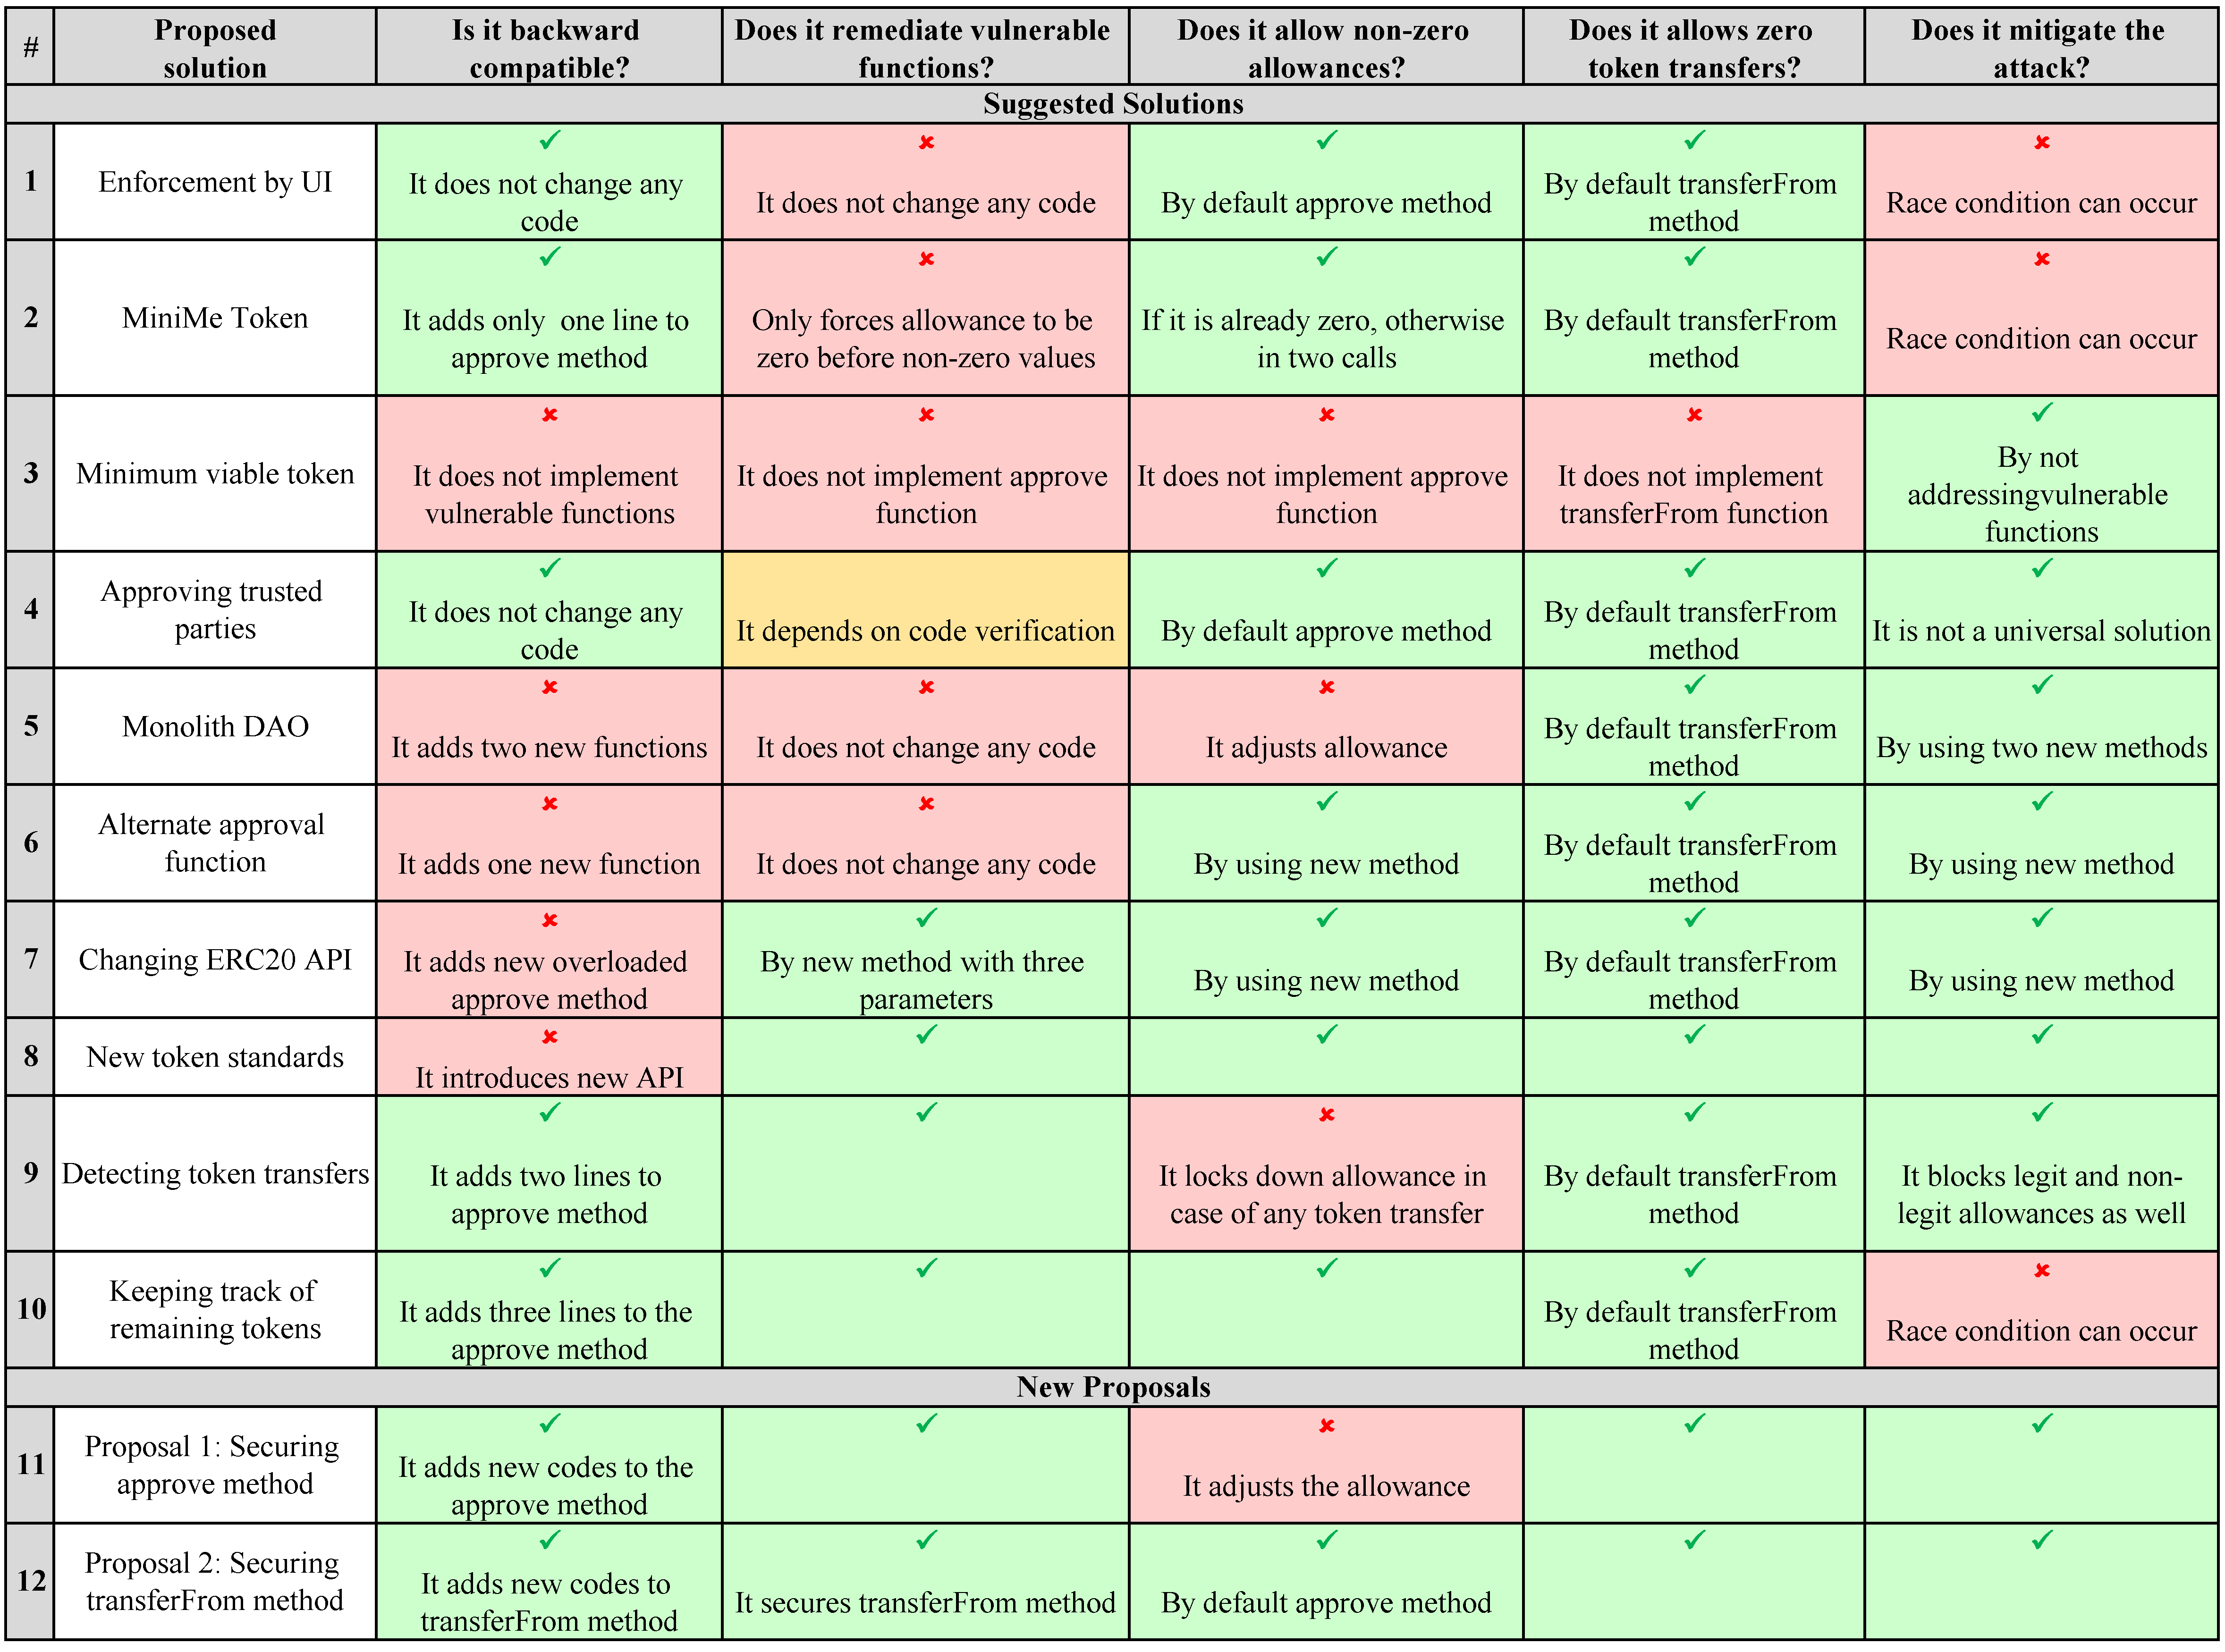
\includegraphics[width=\textwidth]{figures/multiple_withdrawal_04_wide.png}
\caption{Comparison of 10 proposals and 2 contributed by this paper. In our first proposal, CAS is used to mitigate the attack by comparing transferred tokens with new allowance. It is not fully ERC20-compliant since it the allowance result does not always match what is requested. In our second proposal, a new local variable is defined to keep track of transferred tokens and prevents transfers in the case of already transferred tokens.\label{tab:comp}}
\end{figure*}

\subsubsection*{Contributions} In this paper, we evaluate ten proposed mitigations for the multiple withdrawal attack. We develop a set of criteria that encompass backwards compatibility, interoperability, adherence to the ERC20 standard, and attack mitigation. The summary is provided in Figure~\ref{tab:comp}. Since no mitigation is fully satisfactory, we develop two additional solutions based on the \textit{Compare and Set (CAS)} pattern\cite{Ref06}---a widely used lock-free synchronization strategy that allows comparing and setting values atomically. We study in detail possible implementations of ERC20's \texttt{approve} method and \texttt{transferFrom} method. We argue that a CAS-based approach can never adequately deploy a secure \texttt{approve} method while adhering to the ERC20 standard. We then propose a secure implementation of the \texttt{transferFrom} method that mitigates the attack and fully satisfies the ERC20 standard. 

%Finally we note that even if a reader is uninterested in a deep-dive on specific methods within ERC20, this paper has numerous lessons ...

